\documentclass[ignorenonframetext, hyperref=unicode]{beamer}



\usepackage{cmap}
%\usepackage[T2A]{fontenc}
\usepackage[utf8]{inputenc}
\usepackage[bulgarian]{babel}
\selectlanguage{bulgarian}

\usepackage{color}
\usepackage{graphicx}
\usepackage{listings}
\usepackage{rcsinfo}
\usepackage{pgf}
\usepackage{supertabular}
\usepackage{rotating}

\hypersetup{
	colorlinks=true,
	linkcolor=blue,
	filecolor=blue,
	urlcolor=blue,
	anchorcolor=blue,
	citecolor=blue
}

\lstset{language=C++, 
  numbers=left, 
  numberstyle=\tiny,
  stepnumber=1, 
  numbersep=3pt, 
  tabsize=2, 
  texcl,
  basicstyle=\ttfamily\small,
  identifierstyle=\ttfamily\small,
  keywordstyle=\sffamily\bfseries\small,
  extendedchars=true, inputencoding=utf8,
  backgroundcolor=\color[rgb]{1,1,0.845},
  escapeinside={/*@}{@*/}}

%\usepackage{algpseudocode}
%\usepackage[ruled]{algorithm}

\newcommand{\Cpp}{{\ttfamily\bfseries C++}}
\newcommand{\CC}{{\ttfamily\bfseries C}}

\definecolor{outputcolor}{rgb}{0.0,0.0,0.5}
\newcommand{\aout}[1]{\color{outputcolor}{\begin{verbatim}#1\end{verbatim}}}

% \usepackage[T2A]{fontenc}
% \usepackage[cp1251]{inputenc}
% \usepackage[bulgarian]{babel}
\selectlanguage{bulgarian}




\newcommand{\lubo}{%
\author[Л.~Чорбаджиев]{Любомир Чорбаджиев\inst{1} \\ 
{\ttfamily lchorbadjiev@elsys-bg.org}}
\institute[ELSYS] % (optional, but mostly needed)
{
\inst{1}%
Технологическо училище ``Електронни системи'' \\
Технически университет, София
}}

\newcommand{\osauthors}{%
\author{
	В.Кетипов\\ 
	\and
	Н.Димитров \\ 
	\and
	{Х.Стефанов \\
	{\ttfamily elsys.os.2014@gmail.com}}
}
\institute[ELSYS] % (optional, but mostly needed)
{
\inst{1}%
Технологическо училище ``Електронни системи'' \\
Технически университет, София
}}

\titlegraphic{\href{http://creativecommons.org/licenses/by-sa/3.0/}{
\includegraphics{../macros/cc.png}}}

\newcommand{\ie}{т.~е.\ }

\newcounter{probcounter}[section]
\newenvironment{prob}[1][]%
        {\smallskip%
         \noindent\refstepcounter{probcounter}%
          \textbf{\theprobcounter${}^{#1}$.}\ }%
   {\medskip}

\mode<article>
{

}

\mode<presentation>
{
  \usetheme[secheader=true]{Madrid}
  \usecolortheme{crane}
  \usefonttheme[onlylarge]{structurebold}
  \setbeamercovered{transparent}
}

\usepackage[unicode]{hyperref}

%%% Local Variables: 
%%% mode: latex
%%% TeX-master: t
%%% End: 


\title[Файлови Системи]{Файлови Системи} 
\osauthors
\date{\today}

\begin{document}

\frame{\maketitle}

\begin{frame}
\frametitle{Съдържание}
\tableofcontents %[hideallsubsections]
\end{frame}

%-------------------------------------------------------------------- SECTION -
\section{Въведение}

%---------------------------------------------------------------------- SLIDE -
\begin{frame}
\frametitle{Въведение}
\begin{itemize}
  \item Освен енергозависимата памет, често се използва и енергонезависима памет
  \item При енергонезависимата памет съществуват подобни проблеми както при енергозависимата памет:
  \begin{itemize}
    \item Производителност
    \item Защита на паметта
    \item Фрагментация
  \end{itemize}
\end{itemize}
\end{frame}

%-------------------------------------------------------------------- SECTION -
\section{Логическа организация}

%---------------------------------------------------------------------- SLIDE -
\begin{frame}
\frametitle{Въведение}
\begin{itemize}
  \item Една енергонезависима памет може да се разглежда като последователност от байтове
  \item Често те се групират в блокове (твърди дискове, SSD)
  \item При всяко записване или четене от тази памет трябва да укажем къде в паметта искаме да пишем/четем.
  \item Трябва да следим дали не пишем върху памет, която вече е била използвана за други данни
\end{itemize}
\end{frame}

%---------------------------------------------------------------------- SLIDE -
\begin{frame}
\frametitle{Файлове}
\begin{itemize}
  \item За улеснение на потребителите операционната система групира тези последователности от байтове във логическата единица {\em файл}
  \item Това ни позволява да дадем име на тази последователност от байтове
  \item Когато операционната система знае кои байтове на кой файл принадлежат, тя може да гарантира, че един файл не пише върху данните на друг
\end{itemize}
\end{frame}

%---------------------------------------------------------------------- SLIDE -
\begin{frame}
\frametitle{Файлова система}
\begin{itemize}
  \item Файловата система се грижи да организира файловете
  \item Тя следи къде има свободно място върху паметта и коя част от паметта на кой файл принадлежи
\end{itemize}
\end{frame}


%-------------------------------------------------------------------- SECTION -
\section{Oрганизация на файловата система}


%---------------------------------------------------------------------- SLIDE -
\begin{frame}
\frametitle{Директории}
\begin{itemize}
  \item В повечето файлови системи е възможно организирането на група от файлове в директория
  \item Това ни позволява да държим заедно файловете, които имат логическа връзка помежду си
\end{itemize}
\end{frame}

%---------------------------------------------------------------------- SLIDE -
\begin{frame}
\frametitle{Плоска файлова система}
\begin{itemize}
  \item Не съдържа поддиректории. 
  \item Всички файлове се намират в една обща директория, наречена заглавна директория.
\end{itemize}
\begin{figure}[h]
\center
\scalebox{0.315}{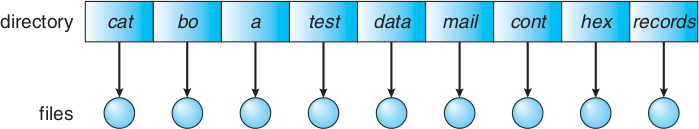
\includegraphics{pics/single_level.png}}
\caption{Silberschatz, Gavin, Gagne: {\em Operating Systems Concepts}}
\end{figure}
\end{frame}

%---------------------------------------------------------------------- SLIDE -
\begin{frame}
\frametitle{Йерархична структура с фиксиран брой нива}
\begin{figure}[h]
\center
\scalebox{0.315}{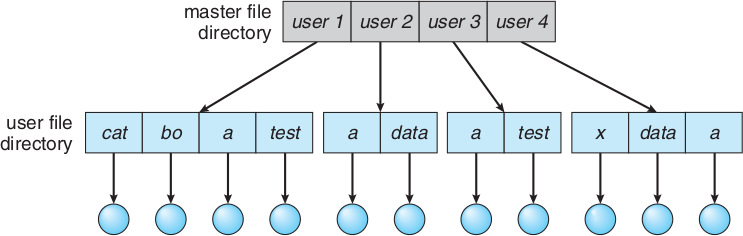
\includegraphics{pics/two_levels.png}}
\caption{Silberschatz, Gavin, Gagne: {\em Operating Systems Concepts}}
\end{figure}
\end{frame}

%---------------------------------------------------------------------- SLIDE -
\begin{frame}
\frametitle{Йерархична структура с произволен брой нива}
\begin{figure}[h]
\center
\scalebox{0.315}{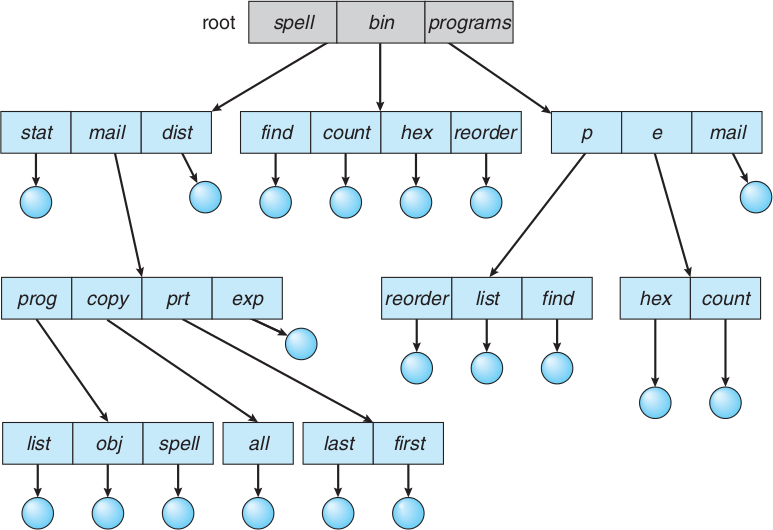
\includegraphics{pics/tree_structure.png}}
\caption{Silberschatz, Gavin, Gagne: {\em Operating Systems Concepts}}
\end{figure}
\end{frame}

%-------------------------------------------------------------------- SECTION -
\section{Пътища}

%---------------------------------------------------------------------- SLIDE -
\begin{frame}
\frametitle{Пътища}
\begin{itemize}
  \item За да намерим даден файл трябва да знаем къде в йерархията се намира
  \item Идентификаторът указващ уникалното местоположение на файл или директория във файловата система се нарича {\em път}
  \item Примери за {\em абсолютен път}:
  \begin{itemize}
    \item /var/log/apache2/access.log
    \item C:\textbackslash Data\textbackslash  Movies\textbackslash movie.mkv
  \end{itemize}
  \item Пътищата може и да са {\em относителни(релативни)} спрямо текущата директория. Пример:
  \begin{itemize}
    \item ../../log/apache2/access.log
    \item a.txt
  \end{itemize}
\end{itemize}
\end{frame}

%-------------------------------------------------------------------- SECTION -
\section{Права}

%---------------------------------------------------------------------- SLIDE -
\begin{frame}
\frametitle{Права}
\begin{itemize}
  \item Модерните операционни системи поддържат множество потребители
  \item Всеки потребител има файлове, които трябва да бъдат достъпни само за него (например: пароли)
  \item Съществуват файлове, които трябва да са достъпни за множество от потребители или за всички
  \item Операционната система трябва да има възможност да ограничава достъпа до дадени файлове
\end{itemize}
\end{frame}

%---------------------------------------------------------------------- SLIDE -
\begin{frame}
\frametitle{Потребители и групи}
\begin{itemize}
  \item За да се улесни управлението на правата, потребителите се разделят в {\em групи}
  \item Всеки потребител може да членува в няколко групи
\end{itemize}
\end{frame}

%---------------------------------------------------------------------- SLIDE -
\begin{frame}
\frametitle{Unix права}
\begin{itemize}
  \item В Unix-базираните операционни системи всеки файл има собственик и асоциирана група
  \item Не е задължително собственикът да е член на асоциираната група
  \item Собственикът може да променя правата върху дадения файл
\end{itemize}
\end{frame}

%---------------------------------------------------------------------- SLIDE -
\begin{frame}
\frametitle{Unix права}
\begin{itemize}
  \item За всеки файл има три вида права:
  \begin{itemize}
	\item Права на собственика
	\item Права на групата
	\item Права на всички останали
  \end{itemize}
  \item Ако даден потребител е собственик на файла, то се гледат правата за собственик
  \item Ако даден потребител е член на групата на файла, то се гледат правата за групата
  \item Ако нито едно от двете не е изпълнено, то се взимат предвид правилата за всички останали
\end{itemize}
\end{frame}


%---------------------------------------------------------------------- SLIDE -
\begin{frame}
\frametitle{Unix права}
\begin{itemize}
  \item Правата биват:
  \begin{itemize}
	\item Права за четене
	\item Права за писане
	\item Права за изпълнение
  \end{itemize}
  \item Дори да сме собственици на даден файл, не е задължително да имаме права върху него. Разбира се, имаме право да ги променим.
\end{itemize}
\end{frame}

%---------------------------------------------------------------------- SLIDE -
\begin{frame}
\frametitle{Unix права}
\begin{figure}[h]
\center
\scalebox{0.315}{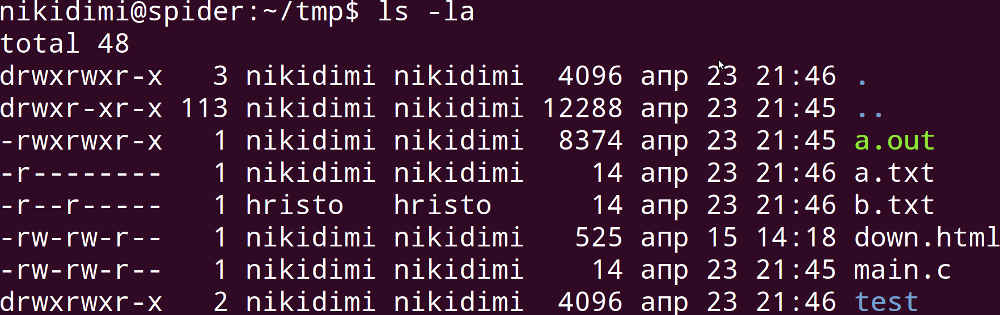
\includegraphics{pics/permissions.png}}
\end{figure}
\end{frame}

%-------------------------------------------------------------------- SECTION -
\section{Физическа организация на файлова система}

%---------------------------------------------------------------------- SLIDE -
\begin{frame}
\frametitle{Физическа организация на файлова система}
\begin{itemize}
  \item Ефективност - Файловата система трябва да осигурява бърз достъп до данните и ефективно използване на дисковата памет.
  \item Надеждност и сигурност - Файловата система трябва да е устойчива в условия на конкурентен достъп от много потребители, при възможни срирове и да е защитена от неправомерен достъп.
  \item Мащабируемост - Файловата система трябва да може да работи както на устройства с малък капацитет (16MB), така и на такива с много голям капацитет (1PB = 1000TB)
\end{itemize}
\end{frame}

%---------------------------------------------------------------------- SLIDE -
\begin{frame}
\frametitle{Физическа организация на файлова система}
\begin{itemize}
  \item Подобно на страницирането на оперативната памет, енергонезависимата памет също се разделя на малки фиксирани части (блокове/сектори)
  \item При записването на файл, се използват един или повече от тези блокове
\end{itemize}
\end{frame}

%---------------------------------------------------------------------- SLIDE -
\begin{frame}
\frametitle{Служебна информация за даден файл}
\begin{itemize}
  \item За да достъпим даден файл трябва да знаем върху кои блокове е разположен.
  \item Освен това къде се намира физически на диска, е необходимо да пазим и друга служебна информация за него като:
  \begin{itemize}
		\item тип
		\item права за достъп
		\item дата и час на създаване
		\item големина
  \end{itemize}
  \item Тази информация най-често се пази на специално място на диска.
  \item В UNIX-базираните операционни системи тази служебна информация се нарича inode.
\end{itemize}
\end{frame}

%---------------------------------------------------------------------- SLIDE -
\begin{frame}
\frametitle{Директории}
\begin{itemize}
  \item Директориите в повечето случаи се пазят като специален файл
  \item Всяка директорията трябва да пази информация за всички файлове, които се намират в нея.
  \item Директорията може да се разглежда като таблица със записи.
  \item За всеки файл/директория има запис, съдържащ името на файла, както и указател към блока, съдържащ служебната информация (inode-а) за този файл.
  \item Служебната информация може да се намира и директно в записа за даден файл/директория, например при файловата система FAT.
\end{itemize}
\end{frame}

%---------------------------------------------------------------------- SLIDE -
\begin{frame}
\frametitle{Достъпване на файл}
\begin{itemize}
  \item На специално място на диска е записана информация за главната (root) директория на файловата система.
  \item Използвайки информацията от нея, ние можем да стигнем до директорията, в която се намира файлът, който искаме да достъпим.
  \item Използвайки информацията от тази директория, можем да намерим физическото местоположение на данните на файла.

\end{itemize}
\end{frame}



%---------------------------------------------------------------------- SLIDE -
\begin{frame}
\frametitle{Физическа организация на файлова система}
\begin{itemize}
  \item Има различни начини за разпределяне на блокове за даден файл:
  \begin{itemize}
	\item Последователно разпределение
	\item Разпределение чрез свързан списък
	\item Разпределение чрез индексна таблица
  \end{itemize}
\end{itemize}
\end{frame}

%---------------------------------------------------------------------- SLIDE -
\begin{frame}
\frametitle{Последователно разпределение}
\begin{itemize}
  \item Най-простия начин за разпределение
  \item Всеки файл се записва в последователни блокове
  \item Необходимо е да се помни само от кой блок започва даден файл и колко на брой блокове заема
\end{itemize}
\end{frame}

%---------------------------------------------------------------------- SLIDE -
\begin{frame}
\frametitle{Последователно разпределение}
\begin{figure}[h]
\center
\scalebox{0.315}{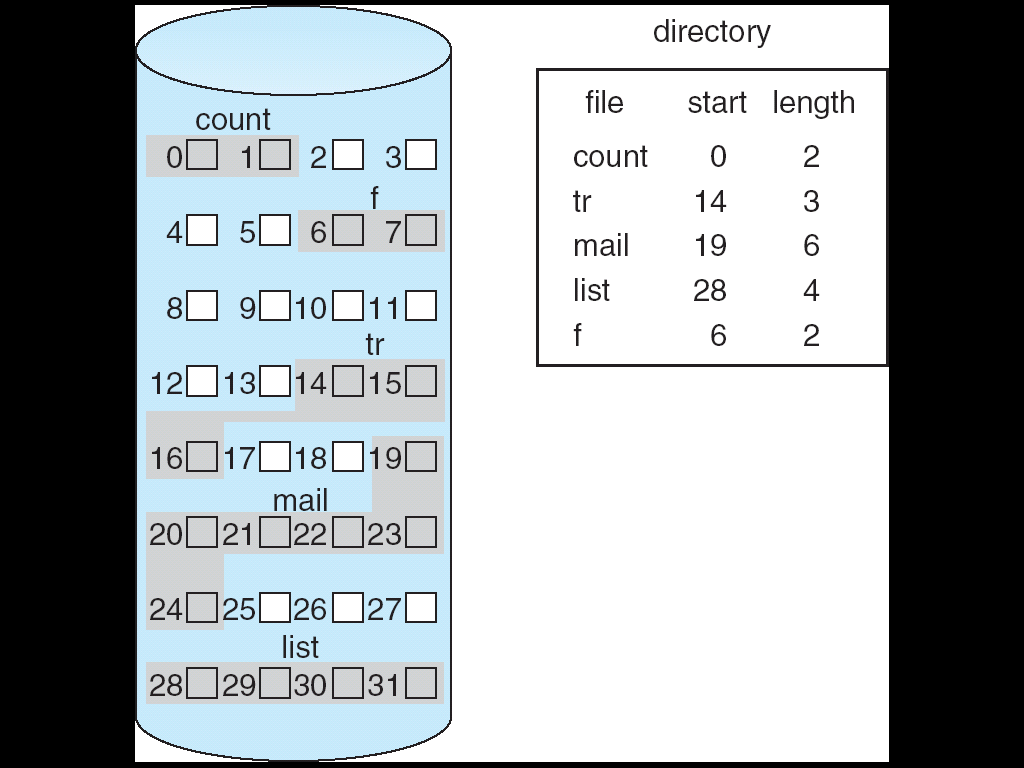
\includegraphics{pics/contiguous_allocation.png}}
\caption{Silberschatz, Gavin, Gagne: {\em Operating Systems Concepts}}
\end{figure}
\end{frame}

%---------------------------------------------------------------------- SLIDE -
\begin{frame}
\frametitle{Предимства и недостатъци}
\begin{itemize}
  \item Бърз достъп до произволна част от файла
  \item Има основни недостатъци:
  \begin{itemize}
	\item Файловете не могат да нарастват, ако блоковете след даден файл са заети
	\item Външна фрагментация - не можем да запазим файл с големина 10 блока, ако например имаме 2 участъка по 5 свободни блока 
  \end{itemize}
\end{itemize}
\end{frame}

%---------------------------------------------------------------------- SLIDE -
\begin{frame}
\frametitle{Разпределение чрез свързан списък}
\begin{itemize}
  \item Всеки файл е разпределен в множество блокове, пръснати из целия диск
  \item Всеки блок пази къде се намира следващия блок от файла, като така образуват свързан списък
\end{itemize}
\end{frame}

%---------------------------------------------------------------------- SLIDE -
\begin{frame}
\frametitle{Разпределение чрез свързан списък}
\begin{figure}[h]
\center
\scalebox{0.315}{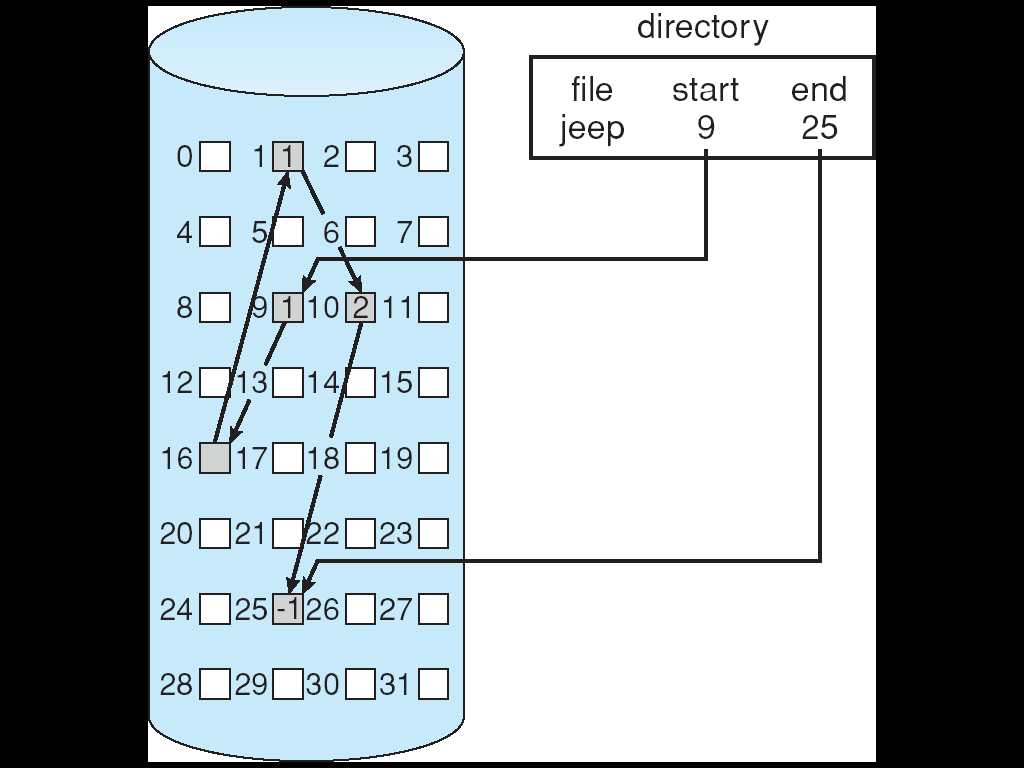
\includegraphics{pics/linked_allocation.png}}
\caption{Silberschatz, Gavin, Gagne: {\em Operating Systems Concepts}}
\end{figure}
\end{frame}

%---------------------------------------------------------------------- SLIDE -
\begin{frame}
\frametitle{Предимства и недостатъци}
\begin{itemize}
  \item Просто за реализация
  \item Необходим е само началния адрес за достъпване на файл
  \item Не страда от външна фрагментация и всички свободни блокове могат да бъдат използвани
  \item Бавен произовлен достъп - трябва да се обходят всички блокове за да се стигне до желания (подобно на търсене в свързан списък)
\end{itemize}
\end{frame}

%---------------------------------------------------------------------- SLIDE -
\begin{frame}
\frametitle{Разпределение чрез индексна таблица}
\begin{itemize}
  \item Всички блокове на даден файл се записват в индексна таблица
  \item Тази таблица се записва в някой свободен блок на диска
\end{itemize}
\end{frame}

%---------------------------------------------------------------------- SLIDE -
\begin{frame}
\frametitle{Разпределение чрез индексна таблица}
\begin{figure}[h]
\center
\scalebox{0.315}{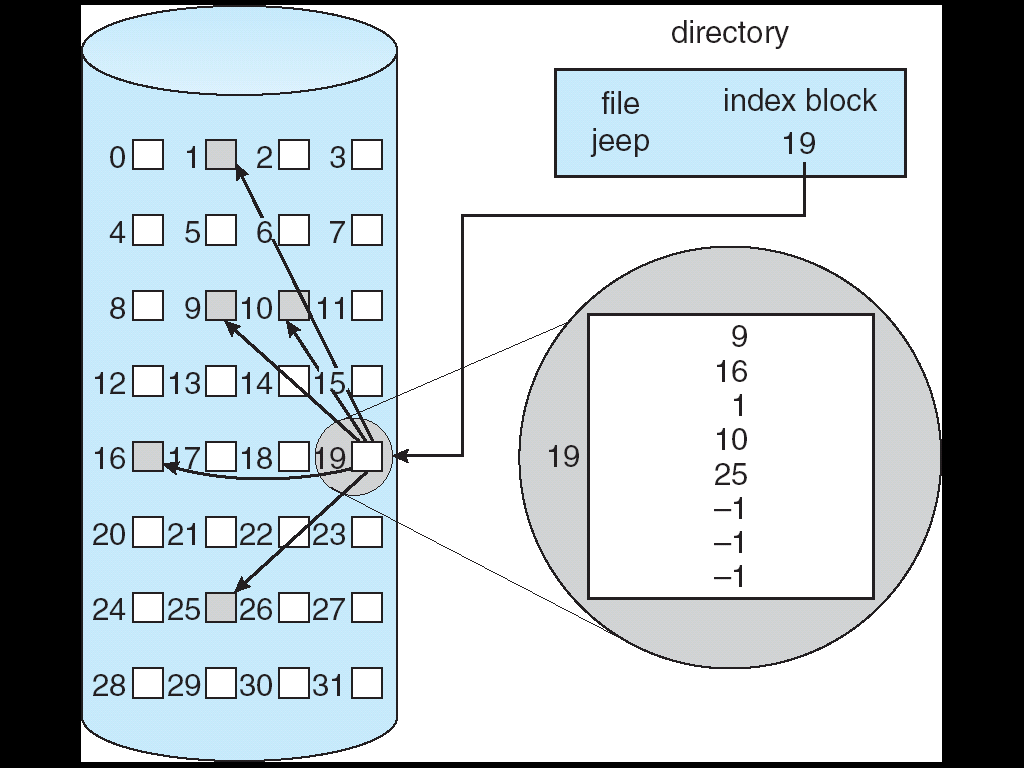
\includegraphics{pics/indexed_allocation.png}}
\caption{Silberschatz, Gavin, Gagne: {\em Operating Systems Concepts}}
\end{figure}
\end{frame}

%---------------------------------------------------------------------- SLIDE -
\begin{frame}
\frametitle{Предимства и недостатъци}
\begin{itemize}
  \item Бърз произволен достъп без външна фрагментация
  \item Необходим е допълнителен блок за индексната таблица
  \item Големината на файла е ограничена от големината на блока, който пази индексната таблица
  \begin{itemize}
		\item Това може да бъде избегнато като се добавят вторични индексни таблици. Така всеки запис в първата индексна таблица сочи към друга индексна таблица, а всеки запис в нея сочи към блок от файла.
		\item При нужда могат да бъдат добавяни и трети, четвърти и т.н. индексни таблици
  \end{itemize}
\end{itemize}
\end{frame}

%---------------------------------------------------------------------- SLIDE -
\begin{frame}
\frametitle{Множество индексни таблици}
\begin{figure}[h]
\center
\scalebox{0.315}{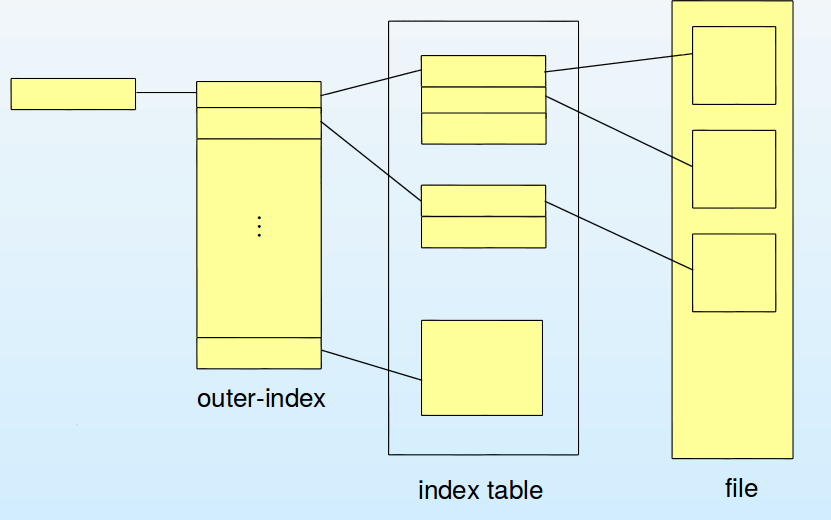
\includegraphics{pics/outer_index.png}}
\caption{Silberschatz, Gavin, Gagne: {\em Operating Systems Concepts}}
\end{figure}
\end{frame}


%---------------------------------------------------------------------- SLIDE -
\begin{frame}
\frametitle{Комбиниран подход}
\begin{figure}[h]
\center
\scalebox{0.315}{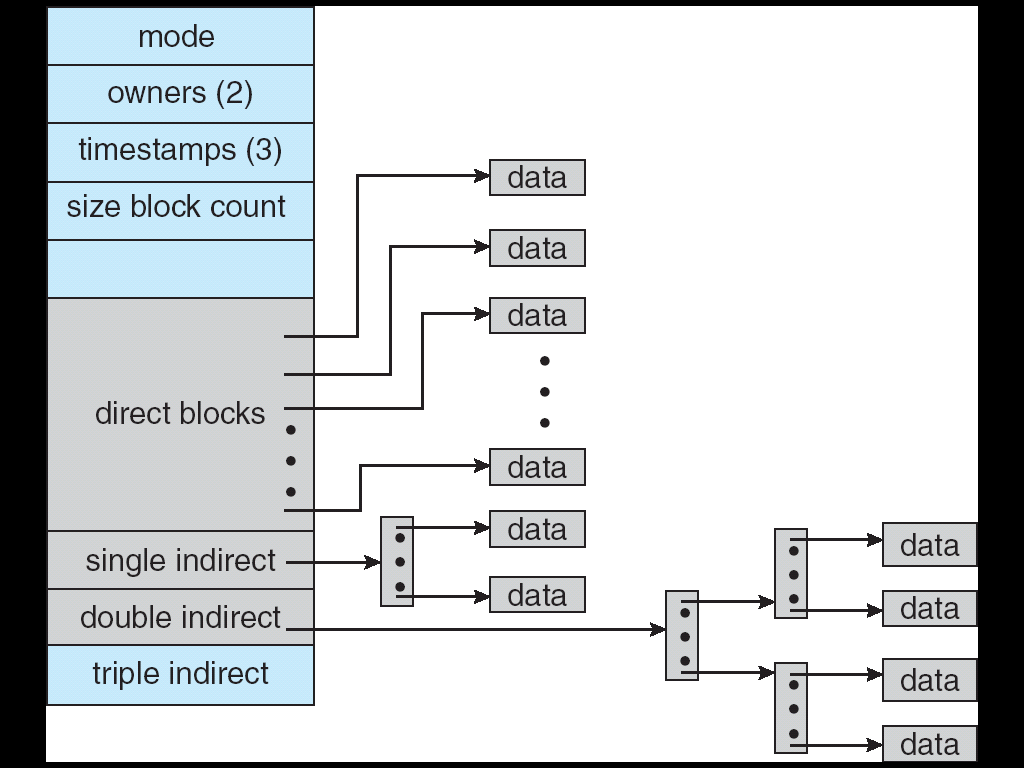
\includegraphics{pics/combined_scheme.png}}
\caption{Silberschatz, Gavin, Gagne: {\em Operating Systems Concepts}}
\end{figure}
\end{frame}

%---------------------------------------------------------------------- SLIDE -
\begin{frame}
\frametitle{Управление на свободното място}
\begin{itemize}
  \item Съществуват два основни подхода:
  \begin{itemize}
		\item Свързан списък от свободни блокове
		\item Побитова карта (bitmap) на свободните блокове
  \end{itemize}
\end{itemize}
\end{frame}

%---------------------------------------------------------------------- SLIDE -
\begin{frame}
\frametitle{Свързан списък от свободни блокове}
\begin{itemize}
  \item Подобно на разпределение чрез свързан списък
  \item Всеки свободен блок пази указател към следващия свободен блок
  \item Необходимо е да знаем само адреса на първия свободен блок
\end{itemize}
\end{frame}


%---------------------------------------------------------------------- SLIDE -
\begin{frame}
\frametitle{Свързан списък от свободни блокове}
\begin{figure}[h]
\center
\scalebox{0.315}{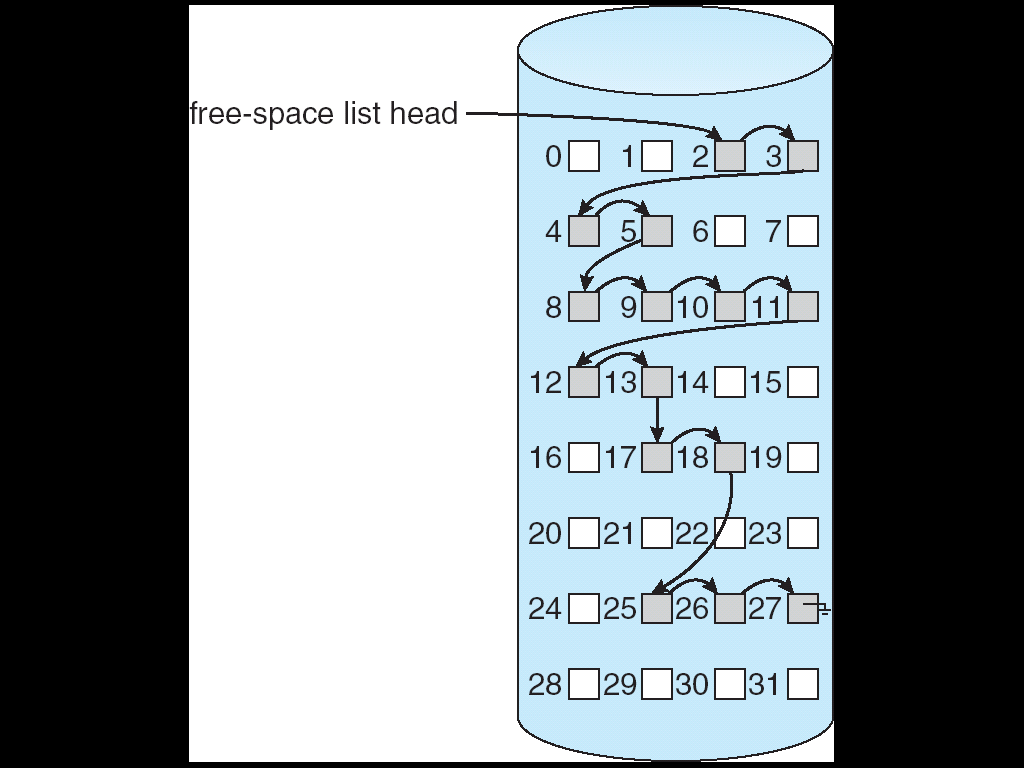
\includegraphics{pics/linked_free_space.png}}
\caption{Silberschatz, Gavin, Gagne: {\em Operating Systems Concepts}}
\end{figure}
\end{frame}

%---------------------------------------------------------------------- SLIDE -
\begin{frame}
\frametitle{Побитова карта (bitmap) на свободните блокове}
\begin{itemize}
  \item Използва се побитова карта, в която за всеки блок от диска има заделен един бит
  \item Стойността на този бит определя дали блокът е зает.
  \item Необходимо е място, където да се запише тази побитова карта
\end{itemize}
\begin{figure}[h]
\center
\scalebox{0.315}{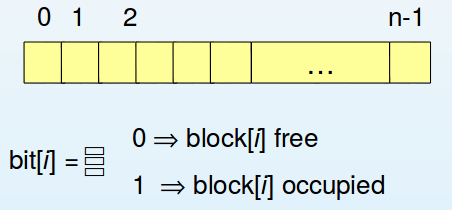
\includegraphics{pics/bitmap_freespace.png}}
\caption{Silberschatz, Gavin, Gagne: {\em Operating Systems Concepts}}
\end{figure}
\end{frame}


%-------------------------------------------------------------------- SECTION -
\section{FAT}


%---------------------------------------------------------------------- SLIDE -
\begin{frame}
\frametitle{FAT}
\begin{itemize}
  \item Паметта се разделя на парчета с фиксиран размер, наречени клъстъри (cluster). Това е най-малката единица, която може да се задели за файл или директория
  \item Използва се разпределение чрез свързан списък
  \begin{itemize}
    \item Един файл може да се съдържа в един или повече клъстери
    \item Всеки клъстър съдържа указател към следващия клъстър от файла или специален указател за край
  \end{itemize}
\end{itemize}
\end{frame}

%---------------------------------------------------------------------- SLIDE -
\begin{frame}
\frametitle{File Allocation Table}
\begin{itemize}
  \item За да се определи състоянието на всеки клъстър, се използва специална таблица.
  \item Тя се нарича File Allocation Table
  \item Представлява разширение на побитовата карта на свободните блокове
  \item Всеки клъстър може да бъде:
  \begin{itemize}
    \item свободен
	\item разпределен за файл
	\item маркиран като повреден
  \end{itemize}
\end{itemize}
\end{frame}

%---------------------------------------------------------------------- SLIDE -
\begin{frame}
\frametitle{Директории}
\begin{itemize}
  \item Директориите се записват като файлове в клъстерите
  \item Тези файлове съдържат таблица, съдържаща запис за всеки файл или поддиректория
  \item Всеки запис в таблицата съдържа: 
  \begin{itemize}
    \item Име на файла
	\item Големина на файла
	\item Дата/час на създаване и последна модификация
	\item Начален клъстър на файла
	\item Права и други атрибути
  \end{itemize}
  \item Главната директория е записана точно след File Allocation Table.
\end{itemize}
\end{frame}


%---------------------------------------------------------------------- SLIDE -
\begin{frame}
\frametitle{File Allocation Table}
\begin{figure}[h]
\center
\scalebox{0.315}{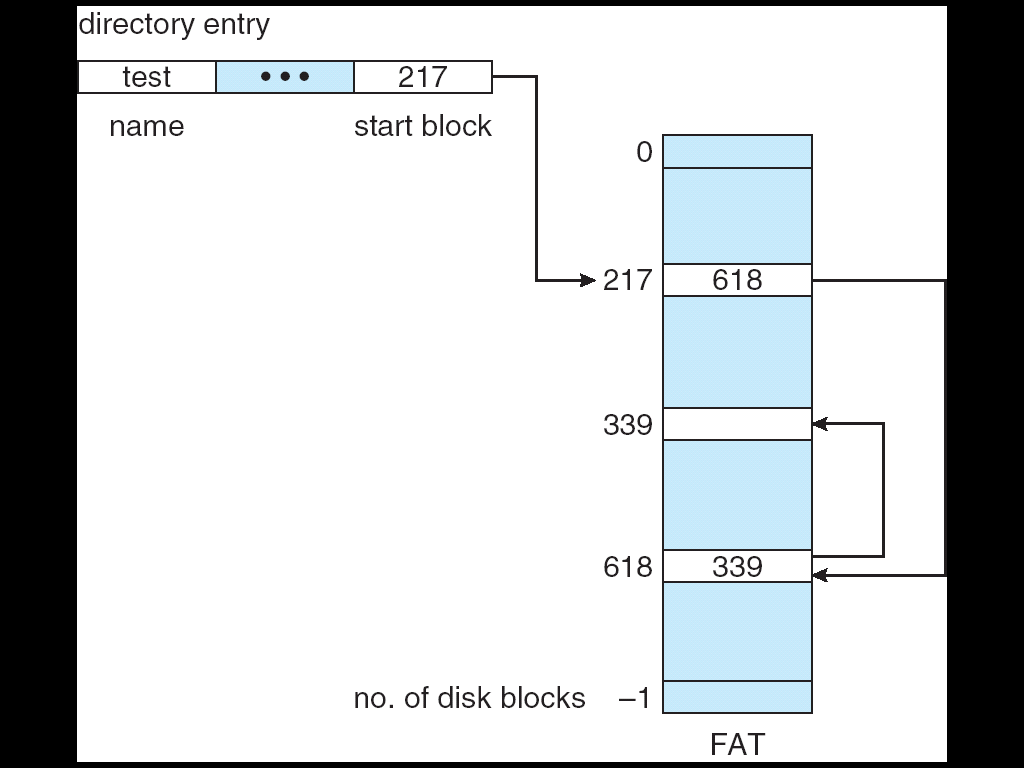
\includegraphics{pics/fat.png}}
\caption{Silberschatz, Gavin, Gagne: {\em Operating Systems Concepts}}
\end{figure}
\end{frame}


\end{document}
